\documentclass[a4paper,twocolumn]{article}

\usepackage{cite}
\usepackage[utf8x]{inputenc}
\usepackage{amsmath}
\usepackage{graphicx}
\usepackage{hyperref}
\usepackage[colorinlistoftodos]{todonotes}

\title{Optimizing SchemaAnalyst Parameter Usage with \texttt{SPOT}}
\author{Nathaniel Blake \\ \textit{Department of Computer Science} \\ \textit{Allegheny College} \and Colin Soleim \\ \textit{Department of Computer Science} \\ \textit{Allegheny College}}
\date{}

\begin{document}

\maketitle

\section{Introduction}

The parameters of a system can play a large role in every aspect of its performance, but they are often set or changed based only on loose testing. Parameter optimization is an attempt to create an experiment to look through a more complete list of possible configurations and accordingly tune a system. The method of sequential parameter optimization has been a popular framework to use since its introduction by Bartz-Beielstein in 2006. Shortly after his initial paper was published, he followed up with a package for R known as the Sequential Parameter Optimization Toolbox or SPOT. This can be found on the Complete R Archive Network website at http://cran.r-project.org/web/packages/SPOT/index.html. 

Our experiment uses this R package to test the parameters of a new system created by Kapfhammer, McMinn, and Wright known as SchemaAnalyst which is built for schema testing. The tool works like this

The four key parameters in SchemaAnalyst are satisfyrows, negaterows, randomprofile, and maxevaluations. These correspond to 

To test the parameters of SchemaAnalyst, we compiled a list of 20 schemas with varying number of constraints and complexity. We ran SPOT with each of these schemas while varying the parameters as stated above. For our performance metric, we created a function that output the expression $ \big( 1 - \frac{\text{Number of Mutants Killed}}{\text{Number of Mutants Created}} \big). $

The results of our experiment revealed that 

Therefore the contributions of this experiment are:

\begin{enumerate}
\item
\item
\item
\end{enumerate}

\section{SPOT} \label{sec:SPOT}

TODO: Description of how SPOT works

\section{SchemaAnalyst} \label{sec:schemaanalyst}

TODO: Full Description of how SchemaAnalyst works

\section{Description of Experiment Design} \label{sec:exp-des}

The core experiment in our research follows the standard use model for SchemaAnalyst, beginning with $(1)$ generation of a set $D$ of database interactions that either satisfy or negate a provided schema $S$ and then $(2)$ running mutation analysis in which the interactions in $D$ are used to try to kill a series of mutant schemas, $S'_1, \dots, S'_n$.

In particular, our \texttt{experiment.R} code uses \texttt{SPOT} to generate parameter designs that include the following four parameters:
\begin{enumerate}
\item \texttt{satisfyrows}, the number of database interactions that satisfy the original schema's constraints,
\item \texttt{negaterows}, the number of database interactions that violate the original schema's constraints in at least one way,
\item \texttt{randomprofile}, a value of either \texttt{'large'} or \texttt{'small'} that determines the scope considered during AVM restarts, and
\item \texttt{randomseed}, a number used to seed the AVM's decisions when using random restart, as well as the seed to the \texttt{Random} generator.
\end{enumerate}

There are two important additional parameters to the generation phase that are not included in our usage of SPOT. The first, \texttt{datagenerator}, is specified by the user at the time of experiment configuration and determines the generator that is used for the entirety of the experiment run's evaluations. The other, \texttt{maxevaluations}, is statically set to an arbitrarily high value of $1,000,000$, since low values are sure to prevent the experiment from producing useful results (because generation will be terminated before the requested number of statements has been created) but higher values are only better to the extent that they do not prevent generation from terminating unnecessarily.

Once \texttt{SPOT} has created a parameter configuration, SchemaAnalyst's \texttt{GenerateResultsFromGenerator} is executed with the provided parameters, and its execution time is measured as a secondary optimization target for \texttt{SPOT}. Once generation is complete, SchemaAnalyst's \texttt{Original} mutation analysis is used against the generated database interactions; \texttt{Original} was chosen because it provides the most comprehensive coverage of mutant types among available techniques, even though it is not as well optimized as others. Follow mutation analysis, the mutation score is recorded, and its inverse is provided to \texttt{SPOT} as the primary optimization target (we use its inverse, calculated as $1 - \frac{\text{Killed Mutants}}{\text{Total Mutants}}$ since \texttt{SPOT} always optimizes using minimization).

From here, \texttt{SPOT} proceeds as described in Section~\ref{sec:SPOT} and in \cite{SPOT2005}, calculating the relative importance of each of the parameters using \texttt{RandomForest} prediction and optimizing its design accordingly over a number of evaluations defined during experiment configuration, storing the mutation score and generation time for each of the configurations that it has tried for later analysis.

\section{Preliminary Analysis of Results}

In our first round of comprehensive data collection and analysis, we ran our experiment with $8$ different schemas of varying complexity (listed in~\nameref{appA}), for each using both \texttt{alternatingValue} and \texttt{alternatingValueDefaults} generators. Before proceeding to analysis, we removed result sets in which every parameter configuration resulted in a mutation score of $1$---at the time being, these data sets obstruct the function of our analysis tools (the use of \texttt{RandomForest}, in particular).

%TODO add citation to compute.es documentation to show how effect size is calculated here
The most general measure of the result sets is the \textit{effect size}, a measure of the strength of the relationship between the mutation scores generated using default parameter values and those generated using optimal parameter configurations determined by \texttt{SPOT} experimentation. For our set of $12$ result sets, the computed Cohen's $d$ value is $0.76$, indicating that there is a relatively strong positive correlation between using optimized parameter values and getting a higher mutation score.

\begin{figure}[t]
\begin{center}
%TODO generate graphics specifically for use in the LaTeX document that are easier to see, sans title
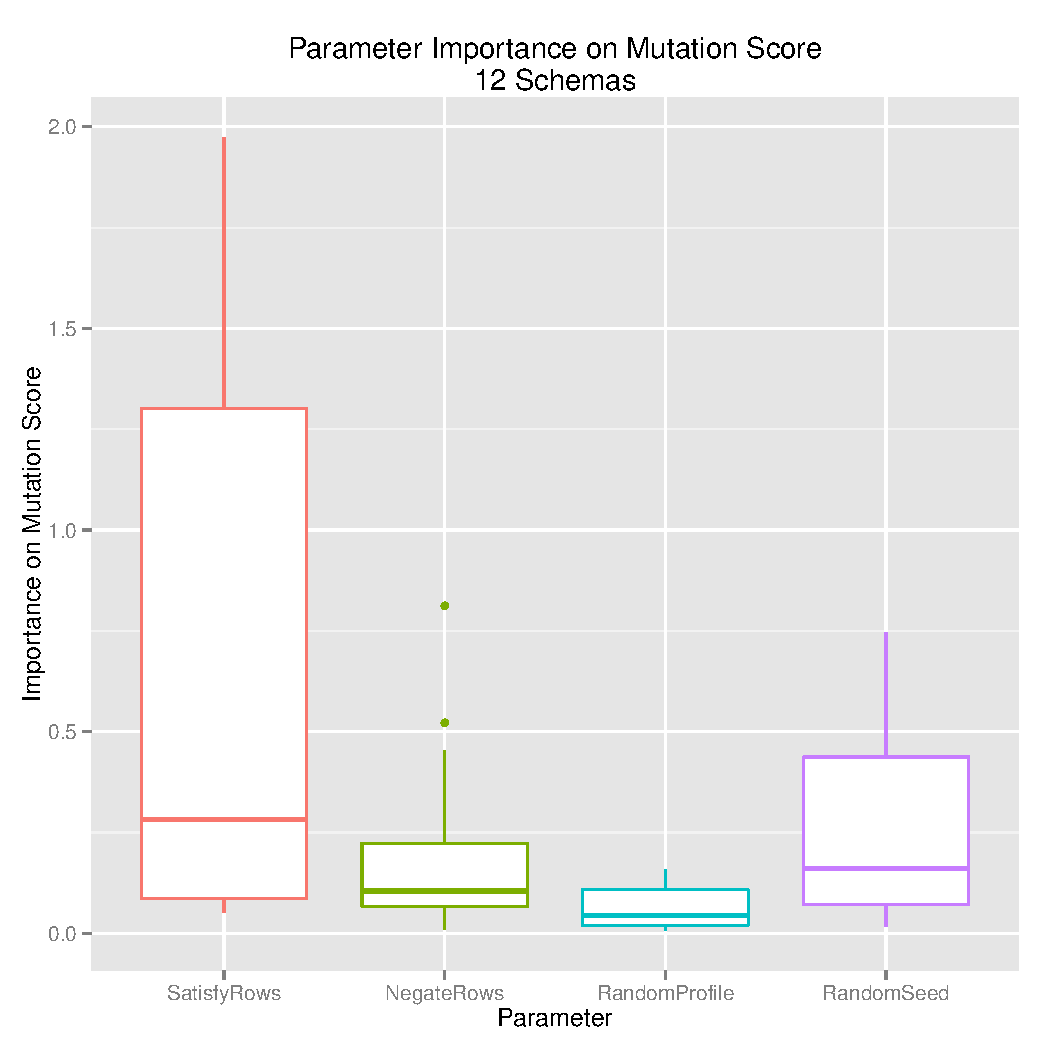
\includegraphics[width=0.90\columnwidth]{mutation-score-importance.pdf}
\caption{Parameter importance on mutation score}
\end{center}
\label{fig:mut-param-imp}
\end{figure}

A similarly broad analysis measures the relative importance of each parameter that is being optimized (refer to~\nameref{sec:exp-des} for parameter descriptions) relative to one of the optimization targets. For instance, Figure~\ref{fig:mut-param-imp} shows that \texttt{SatisfyRows} has the greatest effect on the mutation score, with \texttt{RandomSeed} placing as next most important. This result is reasonable, since a larger number of satisfying database interactions would tailor the set of statements $D$ more closely to the original schema $S$. Then, when $S$ is mutated to form $S'$, at least one of the statements well-suited to $S$ is likely not to be well-suited to $S'$, especially in the case when complex constraints are modified to form $S'$. Likewise, the minimal importance of $NegateRows$ follows since statements that violate $S$ would require that the precise constraint(s) that they violate be modified in the formation of $S'$; this is unlikely, so having a large number of negating interactions is unhelpful to killing mutant schemas, since they're unlikely to be accepted by any schema related to $S$.

%TODO add similar analysis to above for generation-time-importance.pdf

\begin{figure}[t]
\begin{center}
%TODO generate graphics specifically for use in the LaTeX document that are easier to see, sans title
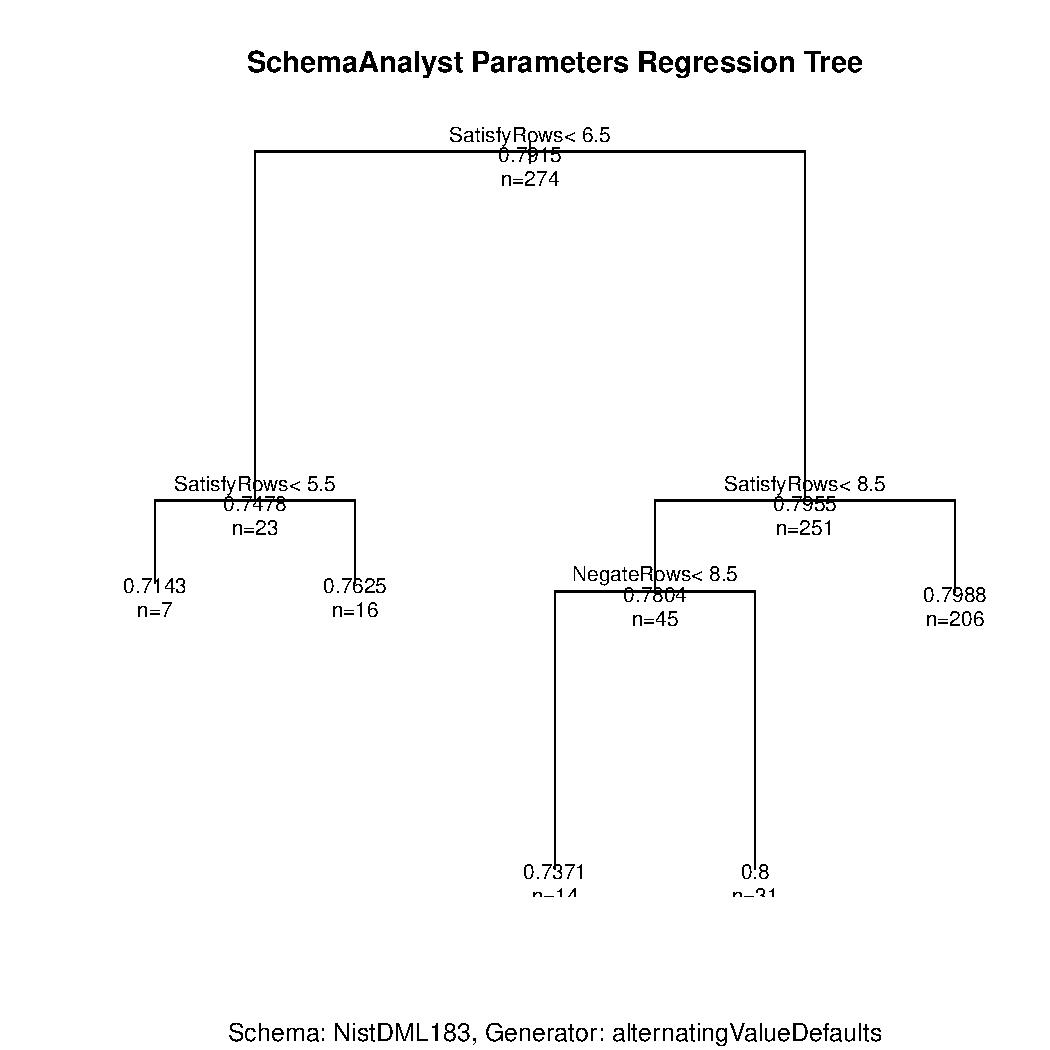
\includegraphics[width=0.90\columnwidth]{NistDML183-regressiontree.pdf}
\caption{Regression tree for NistDML183}
\end{center}
\label{fig:CART}
\end{figure}

We can apply these broad results to analysis of a single result set as well. We see in Figure~\ref{fig:CART} that the first two branches of the classification tree depend on the value of \texttt{SatisfyRows}, again indicative of its correlation to the resultant mutation score; in this case, setting \texttt{SatisfyRows} to $9$ or greater is likely to ensure that the mutation score is near its optimal value in this result set.


\bibliographystyle{acm}
\bibliography{references}

\pagebreak

\section*{Appendix A} \label{appA}
\textit{Listing of schemas tested for preliminary analysis}
\begin{itemize}
\item \texttt{Flights}
\item \texttt{JWhoisServer}
\item \texttt{NistDML181}
\item \texttt{NistDML181NotNulls}
\item \texttt{NistDML182}
\item \texttt{NistDML182NotNulls}
\item \texttt{NistDML183}
\item \texttt{UnixUsage}
\end{itemize}

\end{document}


